\documentclass[11pt,a4paper]{article}
\usepackage[T1]{fontenc}
\usepackage{lmodern,amsmath,amssymb,graphicx,booktabs,tabularx,array,fancyhdr,xcolor,pdfpages}
\usepackage[margin=22mm,headheight=14pt]{geometry}
\usepackage[colorlinks=true,linkcolor=blue!40!black,urlcolor=blue!40!black,pdfauthor={Priyansh Rawat, Mayank Sinha and Samarth Bhatnagar},pdftitle={What Quantum Trace Can a Heavy Particle Leave?}]{hyperref}
\setlength{\parindent}{0pt}\setlength{\parskip}{5pt}\renewcommand{\arraystretch}{1.15}
\pagestyle{fancy}\fancyhf{}\fancyhead[L]{\small Curvature--spectator entanglement}\fancyhead[R]{\small QFT Project B}\fancyfoot[C]{\thepage}
\newcommand{\dd}{\mathrm d}
\newcommand{\avg}[1]{\left\langle #1\right\rangle}
\newcommand{\fig}[3]{\begin{figure}[!ht]\centering\includegraphics[width=#2\linewidth]{assets/#1.pdf}\caption{#3}\end{figure}}
\newcommand{\source}[2]{\par\smallskip{\small\textit{Numerical record.} \href{https://github.com/rawatpriyansh17/QFT-PROJECT-GROUP-B/tree/f30f373285ae649dc4ac4522c6b2031893efc3cc/step#1/results}{#2}.}\par}

% Original typeset pages are included at their A4 coordinates. pdfpages does
% not carry annotations through, so provide the source links on the same pages.
\newcommand{\reportlink}[5]{\put(#1,-#2){\href{#5}{\phantom{\rule{#3bp}{#4bp}}}}}
\newcommand{\pagelink}[5]{\put(#1,-#2){\hyperlink{page.#5}{\phantom{\rule{#3bp}{#4bp}}}}}
\newcommand{\foundationlinks}{%
  \AtPageUpperLeft{\setlength{\unitlength}{1bp}%
  \ifcase\value{page}%
  \or % Foundation page 1
  \or % Foundation page 2
  \or % Foundation page 3
  \or % Foundation page 4
  \or % Foundation page 5
    \pagelink{333.36}{252.53}{7.45}{12.90}{3}%
    \pagelink{387.48}{252.53}{12.90}{12.90}{3}%
    \pagelink{175.15}{434.65}{7.45}{12.90}{2}%
    \pagelink{435.27}{611.05}{7.45}{8.86}{9}%
    \pagelink{447.39}{611.05}{7.45}{8.86}{9}%
  \or % Foundation page 6
    \pagelink{515.31}{77.05}{12.90}{12.90}{5}%
    \pagelink{129.85}{465.12}{12.90}{12.90}{6}%
  \or % Foundation page 7
    \pagelink{415.44}{707.98}{12.90}{12.90}{5}%
  \or % Foundation page 8
    \put(62,-621){\begin{minipage}[t]{165mm}
The single-field and oscillator checks are in \href{https://github.com/rawatpriyansh17/QFT-PROJECT-GROUP-B/blob/main/calculations.py}{\texttt{calculations.py}}. From the repository root, run
\begin{quote}\ttfamily
python3 -m pip install numpy scipy mpmath\\
python3 calculations.py reference
\end{quote}
This writes the analytic reference, finite-difference results and oscillator benchmark to CSV tables in \texttt{results/}. All physical inputs are specified in the script. The archived \href{https://github.com/rawatpriyansh17/QFT-PROJECT-GROUP-B/tree/f30f373285ae649dc4ac4522c6b2031893efc3cc/step1/results}{original validation tables} record the checks used for this section.
\end{minipage}}%
  \or % Foundation page 9
    \reportlink{143.65}{311.85}{105.05}{11.96}{https://arxiv.org/abs/astro-ph/0210603}%
    \reportlink{129.20}{344.72}{105.05}{11.96}{https://arxiv.org/abs/astro-ph/0407059}%
  \or % Foundation page 10
  \or % Foundation page 11
    \pagelink{311.10}{101.62}{7.56}{12.90}{11}%
    \reportlink{461.46}{756.77}{71.62}{11.96}{https://arxiv.org/abs/1110.3234}%
    \reportlink{213.98}{782.65}{81.83}{11.74}{https://github.com/rawatpriyansh17/QFT-PROJECT-GROUP-B/tree/f30f373285ae649dc4ac4522c6b2031893efc3cc/step2}%
  \or % Foundation page 12
  \or % Foundation page 13
  \or % Foundation page 14
    \pagelink{154.12}{77.05}{12.90}{12.90}{13}%
    \reportlink{213.98}{782.65}{81.83}{11.74}{https://github.com/rawatpriyansh17/QFT-PROJECT-GROUP-B/tree/f30f373285ae649dc4ac4522c6b2031893efc3cc/step3}%
  \or % Foundation page 15
  \or % Foundation page 16
  \or % Foundation page 17
    \pagelink{96.01}{755.55}{7.49}{11.63}{18}%
  \or % Foundation page 18
    \pagelink{94.73}{109.52}{7.34}{11.63}{19}%
  \or % Foundation page 19
  \or % Foundation page 20
    \pagelink{97.41}{403.78}{7.56}{11.63}{20}%
    \pagelink{493.46}{403.78}{7.56}{11.63}{21}%
  \or % Foundation page 21
    \pagelink{354.28}{388.04}{7.45}{11.63}{21}%
  \or % Foundation page 22
  \or % Foundation page 23
  \or % Foundation page 24
  \or % Foundation page 25
    \pagelink{95.80}{649.23}{12.90}{11.63}{26}%
  \or % Foundation page 26
  \or % Foundation page 27
  \or % Foundation page 28
  \or % Foundation page 29
  \or % Foundation page 30
  \or % Foundation page 31
    \reportlink{379.32}{471.10}{76.74}{11.95}{https://arxiv.org/abs/1503.08043}%
    \reportlink{213.98}{502.21}{81.83}{11.74}{https://github.com/rawatpriyansh17/QFT-PROJECT-GROUP-B/tree/f30f373285ae649dc4ac4522c6b2031893efc3cc/step6}%
  \fi}}

\begin{document}
\hypersetup{pageanchor=false}
\begin{titlepage}\centering\vspace*{4mm}

\includegraphics[width=35mm]{assets/bits_logo.png}\par\vspace{13mm}
{\Large\bfseries BITS PILANI K.K. BIRLA GOA CAMPUS\par}{\large Department of Physics\par}
\vspace{22mm}{\LARGE\bfseries What Quantum Trace Can\\[2mm] a Heavy Particle Leave?\par}
\vspace{5mm}{\large Curvature--Spectator Entanglement\\and the Cosmological Collider\par}
\vspace{19mm}{\large\bfseries Group B\par}\vspace{3mm}
\begin{tabular}{ll}Priyansh Rawat & 2023B5A70968G\\Mayank Sinha & 2023B5A70942G\\Samarth Bhatnagar & 2023B5A70853G\end{tabular}
\vfill Supervisor: Professor Rudranil Basu\par\smallskip 19 November 2026
\end{titlepage}
\pagenumbering{roman}\hypersetup{pageanchor=true}
\setcounter{tocdepth}{1}\tableofcontents
\vspace{8mm}\textbf{Project result.} In the selected two-field model, tracing out the spectator leaves the light field with a positive Gaussian entropy. A separate cubic coupling controls the leading three-point signal. At fixed mass and mixing we can turn off this signal while keeping the same Gaussian entropy. With the cubic coupling restored, the oscillation across squeezed triangles gives $1.993\leq m/H\leq2.020$ across the tested fit choices at input $m/H=2$.
\clearpage\pagenumbering{arabic}
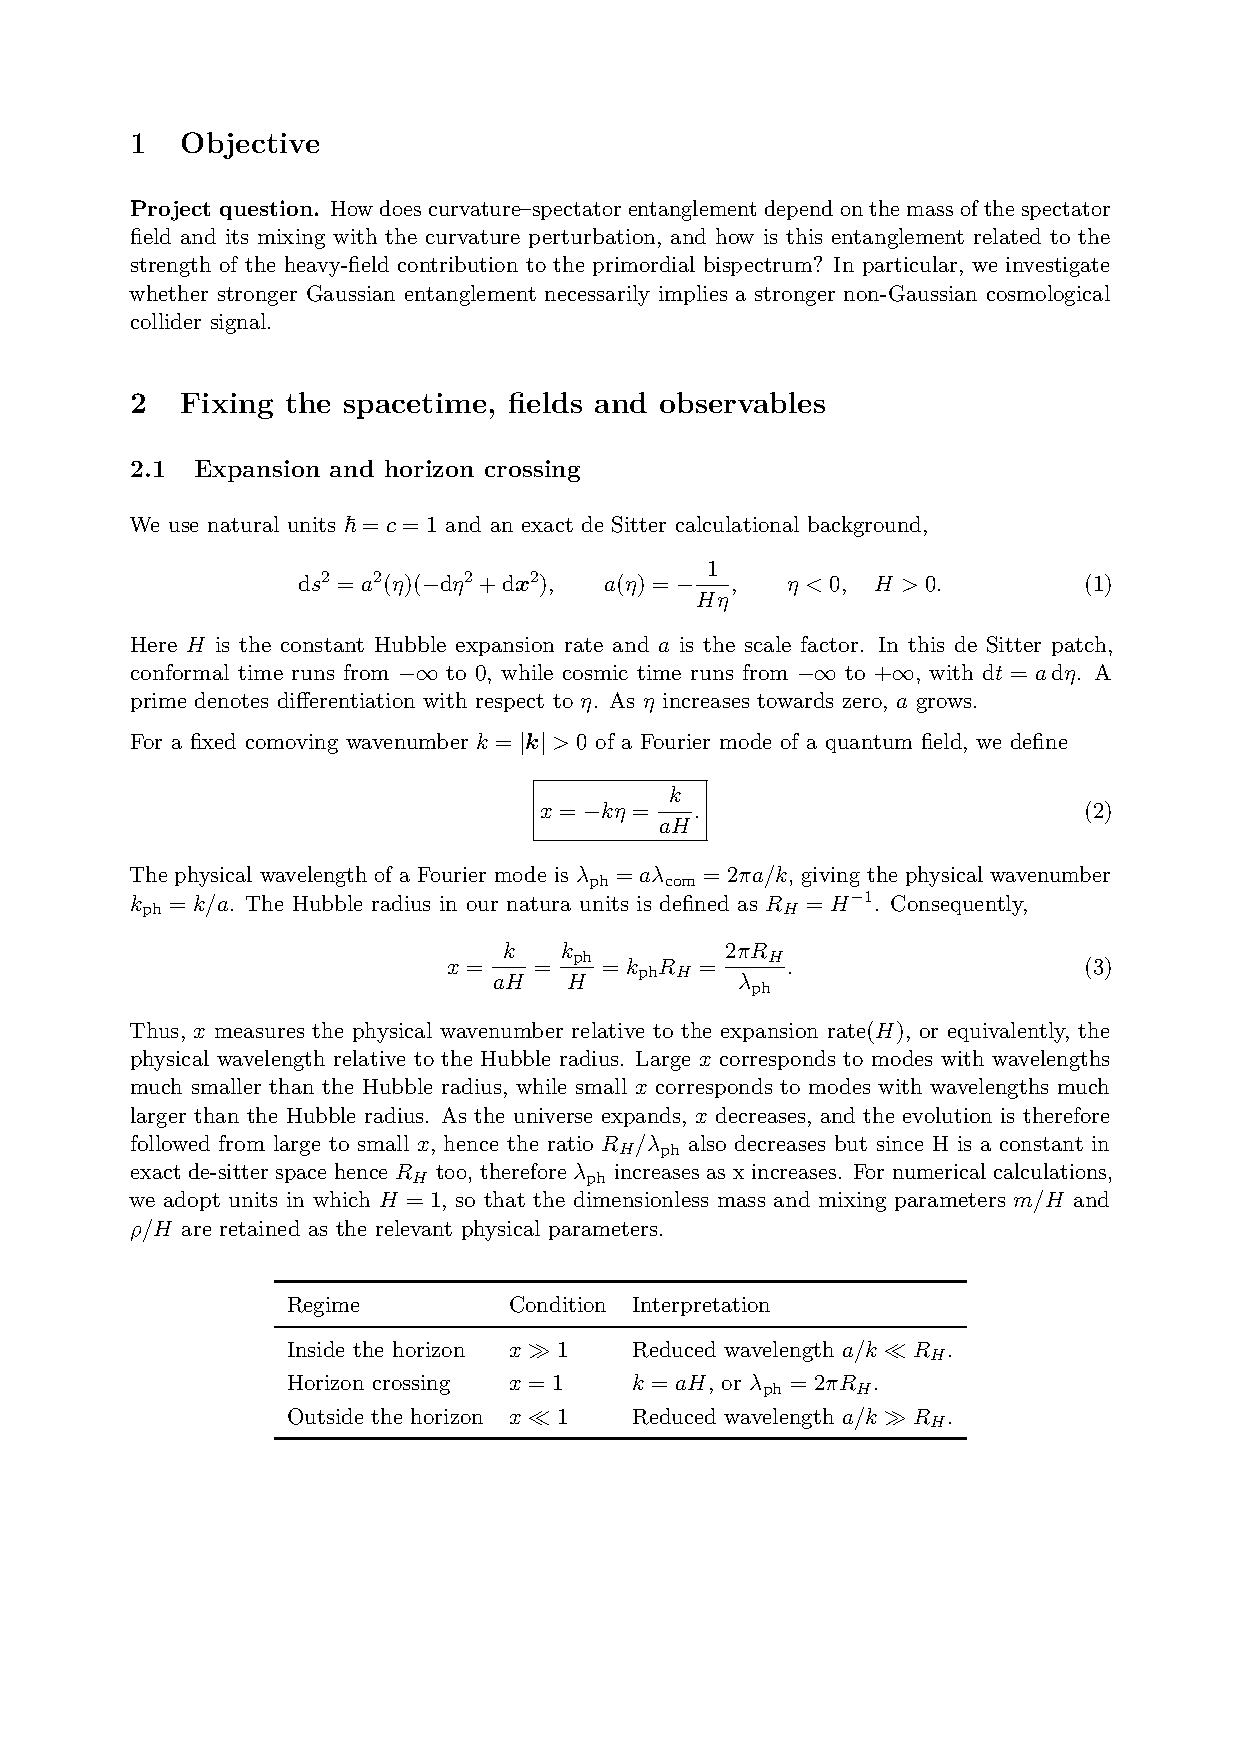
\includepdf[pages=-,pagecommand={\thispagestyle{fancy}\AddToShipoutPictureFG*{\foundationlinks}},addtotoc={
1,section,1,Objective,base:objective,
1,section,1,{Fixing the spacetime, fields and observables},base:fields,
10,section,1,Understanding the entropy with two ordinary oscillators,base:osc,
12,section,1,Deriving the canonical equations before coding,base:canonical,
15,section,1,Initialising and validating the mode functions,base:modes,
23,section,1,Extracting and interpreting the Gaussian entanglement,base:entropy,
30,section,1,Understanding the heavy-field clock and the in-in formula,base:inin}]{assets/foundation.pdf}
\setcounter{section}{7}\setcounter{equation}{118}\setcounter{figure}{14}

% Bispectrum
\section{From the quadratic state to the spectator bispectrum}
\subsection{What is measured at the final time?}
Let $\hat q_{\mathbf k}(\eta_f)$ be the Fourier component of the light-field \emph{operator}. Angular brackets are an expectation in the state evolved from the initial vacuum. With the Fourier convention of Eqs.~(9)--(10),
\begin{align}
\avg{\hat q_{\mathbf k}\hat q_{\mathbf p}}_0
  &=(2\pi)^3\delta^3(\mathbf k+\mathbf p)\,P_q(k;\eta_f),\\
\avg{\hat q_{\mathbf k_1}\hat q_{\mathbf k_2}\hat q_{\mathbf k_3}}_c
  &=(2\pi)^3\delta^3(\mathbf k_1+\mathbf k_2+\mathbf k_3)\,B_q(k_1,k_2,k_3;\eta_f).
\end{align}
All three external fields are evaluated at $\eta_f$. After removing the momentum delta function, $P_q$ is an ordinary, real, nonnegative function of the magnitude $k$ and time. The subscript $0$ specifies the mixed quadratic Gaussian theory. The subscript $c$ retains the connected part. We keep the power at quadratic order and calculate the leading connected $B_q$ to first order in the cubic interaction.

To see precisely what sets the power, write the light and heavy fields with the same two vacuum columns $b=1,2$. For $s=q,\sigma$,
\begin{equation}
\hat s_{\mathbf k}(\eta)=\sum_{b=1}^2
 [s_k^b(\eta)\hat a_b(\mathbf k)+s_k^{b*}(\eta)\hat a_b^\dagger(-\mathbf k)] .
\end{equation}
The only surviving vacuum contraction is
\[\avg{\hat a_b(\mathbf k)\hat a_c^\dagger(-\mathbf p)}_0=(2\pi)^3\delta_{bc}\delta^3(\mathbf k+\mathbf p).\]
Multiplication of the two light-field expansions therefore gives
\begin{equation}
 P_q(k;\eta_f)=\sum_b q_k^b(\eta_f)q_k^{b*}(\eta_f)
 =\frac{H^2}{k^3}\sum_b|Q_b(-k\eta_f)|^2 .
\end{equation}
Here $q_k^b=H k^{-3/2}Q_b$ and $\sigma_k^b=H k^{-3/2}\Sigma_b$. The column amplitudes are complex-valued mode functions. For a free massless field the column sum is $(1+x_f^2)/2$, giving the familiar late-time power $H^2/(2k^3)$.

For a squeezed triangle with $k_1=k_L=r k_S$ and $k_2=k_3=k_S$, define the dimensionless observable
\begin{equation}\boxed{\displaystyle F_q(r)=\frac{H\,B_q(k_L,k_S,k_S;\eta_f)}
 {P_q(k_L;\eta_f)P_q(k_S;\eta_f)}.}\label{eq:shape}\end{equation}
We write $F$ for $F_q$ in plots and numerical tables. Each evaluation gives one real number. The denominator uses the ordinary two-point powers, with one long and one short factor. The factor $H$ removes the inverse field dimension of $B_q/P_q^2$. The dimensionless power per logarithmic interval would instead contain $k^3/(2\pi^2)$. For the conversion $q=C\zeta$ in Eq.~(17), $B_\zeta/(P_{\zeta,L}P_{\zeta,S})=(C/H)F_q$.

\clearpage
\subsection{Where the in-in time integral comes from}
The mixed quadratic Hamiltonian defines the interaction picture. It already evolves the coupled mode functions. The remaining interaction is the cubic Hamiltonian $H_I(\eta)$. Let $\eta_0$ be an early initial time and choose $U_I(\eta_0,\eta_0)=1$. The equation $i\partial_{\eta}U_I=H_I U_I$ integrates to
\begin{equation}
 U_I(\eta_f,\eta_0)=1-i\int_{\eta_0}^{\eta_f}\dd\eta\ H_I(\eta)U_I(\eta,\eta_0).
\end{equation}
Since $H_I$ is already first order in the cubic coupling, replace $U_I$ under the integral by its zeroth-order value $1$. For $A=\int_{\eta_0}^{\eta_f}\dd\eta\ H_I(\eta)$, Hermiticity gives $A^\dagger=A$. Thus $U_I=1-iA+O(\lambda_3^2)$ and $U_I^\dagger=1+iA+O(\lambda_3^2)$. With $O=O_I(\eta_f)$ the multiplication is
\begin{align}
\avg{U_I^\dagger O U_I}_0
 &=\avg{(1+iA)O(1-iA)}_0+O(\lambda_3^2)\nonumber\\
 &=\avg O_0+i\avg{AO}_0-i\avg{OA}_0+O(\lambda_3^2).
\end{align}
Subtract the unperturbed term and use $[O,H_I]=OH_I-H_IO$. The integration sums over every time when the interaction could act before measurement:
\begin{equation}\boxed{\displaystyle
\Delta\avg O=-i\int_{\eta_0}^{\eta_f}\dd\eta\left(\avg{O H_I(\eta)}_0-\avg{H_I(\eta)O}_0\right)
=-i\int_{\eta_0}^{\eta_f}\dd\eta\,\avg{[O,H_I(\eta)]}_0 .}
\end{equation}
Taking the early-time limit with the vacuum regulator gives Eq.~(116). For a Fourier triangle $O^\dagger$ reverses every external momentum. Reality of the fields and parity invariance of this scalar state identify the reduced coefficient for that reversed triangle with the original one. Equivalently, the Wick products in the two orderings below are conjugates. If $Z$ is the coefficient in $\avg{O H_I}_0$, the difference is $Z-Z^*=2i\,\mathrm{Im}\,Z$. Multiplying by $-i$ gives $+2\,\mathrm{Im}\,Z$.

\subsection{Evaluating the benchmark integral in Eq.~(117)}
The test vertex in Section 7 is $\gamma a(q')^3/3!$ in the Hamiltonian density. For a massless mode $u_k(\eta)=H(1+ik\eta)e^{-ik\eta}/\sqrt{2k^3}$, differentiation cancels the two terms proportional to $ik$ and leaves $u'_k=H k^2\eta e^{-ik\eta}/\sqrt{2k^3}$. Each late-to-vertex contraction gives
\[
 u_k(0)u_k^{\prime *}(\eta)=\frac{H^2\eta}{2k}e^{ik\eta}.
\]
Multiplying three contractions produces $H^6\eta^3 e^{iK\eta}/(8k_1k_2k_3)$, with $K=k_1+k_2+k_3$. The factor $a=-1/(H\eta)$ supplies the minus sign and reduces $\eta^3$ to $\eta^2$. The six external-to-vertex pairings cancel $3!$. The commutator then supplies the factor of two in Eq.~(118).
\clearpage
With $s=(\epsilon+i)K$, $\epsilon>0$, the factor $e^{\epsilon K\eta}$ damps the integrand towards $\eta=-\infty$. Write $J_n=\int_{-\infty}^0\eta^n e^{s\eta}\dd\eta$. Since $\mathrm{Re}\,s>0$, every lower boundary term vanishes. Integration by parts gives
\begin{align}
J_0&=[e^{s\eta}/s]_{-\infty}^0=1/s,\nonumber\\
J_1&=[\eta e^{s\eta}/s]_{-\infty}^0-J_0/s=-1/s^2,\nonumber\\
I_\epsilon=J_2&=[\eta^2 e^{s\eta}/s]_{-\infty}^0-2J_1/s=2/s^3.
\end{align}
As $\epsilon\to0^+$ we have $1/i^3=i$, so $\mathrm{Im}\, I_\epsilon\to2/K^3$. Substitution gives
\[B_{\rm test}=-\frac{\gamma H^5}{4 k_1k_2k_3}\frac{2}{K^3}=-\frac{\gamma H^5}{2 k_1k_2k_3 K^3}.\] The test checks the commutator sign independently of the heavy-field evolution.

\subsection{Why one cubic vertex gives three mixed contractions}
For the physical interaction, take $O=\hat q_{\mathbf k_1}\hat q_{\mathbf k_2}\hat q_{\mathbf k_3}$ and $H_I=(\lambda_3/3!)\,a^4\int\dd^3x\,\hat\sigma^3$. All spectator operators are at the integration time $\eta$. Fourier expanding the three fields and integrating over $\mathbf x$ gives
\begin{equation}
 H_I=\frac{\lambda_3 a^4}{3!}\int\prod_{j=1}^3\frac{\dd^3p_j}{(2\pi)^3}\,
 (2\pi)^3\delta^3(\mathbf p_1+\mathbf p_2+\mathbf p_3)
 \hat\sigma_{\mathbf p_1}\hat\sigma_{\mathbf p_2}\hat\sigma_{\mathbf p_3}.
\end{equation}
The same vacuum multiplication used for $P_q$ now pairs two different fields at two different times:
\begin{align}
\avg{\hat q_{\mathbf k}(\eta_f)\hat\sigma_{\mathbf p}(\eta)}_0
 &=(2\pi)^3\delta^3(\mathbf k+\mathbf p)K_k(\eta_f,\eta),\nonumber\\
K_k(\eta_f,\eta)&=\sum_b q_k^b(\eta_f)\sigma_k^{b*}(\eta).
\end{align}
For one connected Wick pairing, $q_1$ pairs with $\sigma_1$, $q_2$ with $\sigma_2$ and $q_3$ with $\sigma_3$. The three delta functions set $\mathbf p_j=-\mathbf k_j$. The vertex delta then imposes $\sum_j\mathbf k_j=0$. There are $3\times2\times1=6$ choices of which spectator each external leg pairs with. Relabeling the dummy momenta gives the same product for all six. Pairing two external legs together gives a disconnected term, excluded from $B_q$.

Stripping off the single remaining delta function yields $Z=(6/3!)\lambda_3 a^4 K_{k_1}K_{k_2}K_{k_3}$. Reversing the operator order conjugates each $K_k$. The commutator found above therefore gives
\begin{equation}\boxed{\displaystyle B_q=2\lambda_3\int_{-\infty}^{\eta_f}\dd\eta\,a^4(\eta)\,
 \mathrm{Im}\!\left[K_{k_1}K_{k_2}K_{k_3}\right].}\end{equation}
Squares of magnitudes discard relative phases. A list of final powers therefore cannot reconstruct this integral.
\clearpage
\subsection{One final time, two momentum scales}
Set $z=-k_S\eta$ and $z_f=-k_S\eta_f$. For the short legs, $-k\eta=z$ and $-k\eta_f=z_f$. On the long leg the same times give $rz$ and $rz_f$. For example, $r=0.03$ and $z_f=0.01$ give long final argument $0.0003$. Evaluating the long leg at $0.01$ would select a different physical time.
\begin{align}
C_L(z)&=\sum_b Q_b(rz_f)\Sigma_b^*(rz), &C_S(z)&=\sum_b Q_b(z_f)\Sigma_b^*(z),\nonumber\\
p_L&=\sum_b|Q_b(rz_f)|^2, &p_S&=\sum_b|Q_b(z_f)|^2.
\end{align}
Each contraction contains two factors of $Hk^{-3/2}$. Thus $K_L=H^2 C_L/k_L^3$, $K_S=H^2 C_S/k_S^3$, $P_L=H^2 p_L/k_L^3$ and $P_S=H^2 p_S/k_S^3$. Here $P_L,P_S$ abbreviate the two evaluations of $P_q$.

Now $a=k_S/(Hz)$ and $\dd\eta=-\dd z/k_S$. Reversing the limits removes the minus sign and gives
\[
 \int_{-\infty}^{\eta_f}\dd\eta\,a^4(\eta)(\cdots)
 =\frac{k_S^3}{H^4}\int_{z_f}^\infty\frac{\dd z}{z^4}(\cdots).
\]
Use this result before setting numerical units:
\begin{align}
 B_q&=2\lambda_3\frac{k_S^3}{H^4}\frac{H^6}{k_L^3 k_S^6}
 \int_{z_f}^\infty\frac{\dd z}{z^4}\,\mathrm{Im}(C_L C_S^2),\nonumber\\
 P_LP_S&=\frac{H^4p_Lp_S}{k_L^3 k_S^3},\nonumber\\
 F_q(r)&=\frac{2(\lambda_3/H)}{p_Lp_S}\int_{z_f}^\infty\frac{\dd z}{z^4}\,
 \mathrm{Im}\!\left[C_L(z)C_S(z)^2\right].
\end{align}
Both the numerator and denominator of Eq.~\eqref{eq:shape} carry $1/(k_L^3k_S^3)$. This cancels the explicit $r^{-3}$ from $k_L=r k_S$ while retaining physical $r$ dependence in the complex modes. The square is an ordinary complex square because there are two short contractions in the same ordering.

\textbf{From the integral to a stored number.} For quadrature nodes $z_j$ and weights $w_j$, store $G_j=C_L(z_j)C_S(z_j)^2/z_j^4$. Since $K\eta=-(2+r)z$, the regulated numerical estimator is
\begin{equation}
 F_{\epsilon,L}=\frac{2(\lambda_3/H)}{p_Lp_S}\sum_{z_j\in[z_f,L]} w_j e^{-\epsilon(2+r)z_j}\,\mathrm{Im}\,G_j .
\end{equation}
$L$ is the integration cutoff. The earlier mode initialisation occurs at $X\ge L$. The vacuum limit requires control of both $L$ and $\epsilon$. Setting $\epsilon=0$ at a fixed small $L$ would expose an unsuppressed oscillatory tail.

\clearpage
\subsection{Pilot signal and coupling controls}
The pilot uses $H=k_S=1$, $M=m/H=2$, $g=0.1$, $\lambda_3/H=0.01$, $X=800$, $z_f=0.01$, $L=320$ and $\epsilon=0.025$. At $r=0.1,0.03,0.01$ the regulated values are respectively $1.92979\times10^{-9}$, $-3.64205\times10^{-10}$ and $5.80157\times10^{-11}$. The sign change motivates scanning the triangle ratio after verifying convergence.
\fig{cumulative_integral}{.82}{Running sum at $r=0.03$, accumulated from late time towards earlier times. The individual lobes are larger than their residual. This cancellation makes the sign and phase of each contraction important.}
\textbf{Two exact zeros.} Setting $\lambda_3=0$ removes the vertex. At $g=0$ the vacuum columns of $q$ and $\sigma$ have disjoint support, so $K_k=0$ on every leg. Both controls return zero. Doubling $\lambda_3/H$ to $0.02$ doubles the pilot result, as required by a first-order calculation.

\textbf{Weak mixing.} Each mixed contraction requires one transfer between the fields and starts at order $g$. Three such contractions give $F\propto\lambda_3 g^3$ at leading weak mixing. The power corrections start at even order. At the same $r=0.03$, the three measurements give
\begin{center}\begin{tabular}{rrr}\toprule $g$ & Regulated $F$ & $F/g^3$ \\\midrule
0.025 & $-5.8382\times10^{-12}$ & $-3.7364\times10^{-7}$\\
0.050 & $-4.6468\times10^{-11}$ & $-3.7175\times10^{-7}$\\
0.100 & $-3.6420\times10^{-10}$ & $-3.6420\times10^{-7}$\\\bottomrule\end{tabular}\end{center}
The small drift in the last column is consistent with the expected departure from leading scaling as mixing increases.
\source{7}{Complex modes, integrand, regulated values and mixing controls}


% Convergence
\clearpage\section{Convergence of the time integral}
\subsection{Separate the integration cutoff from the vacuum regulator}
At fixed $\epsilon>0$ the early-time integrand is damped. Increasing the upper limit $L$ tests how much of that damped tail was omitted. Reducing $\epsilon$ changes the integral itself, so one must extend the integration far enough to resolve the slower damping. These two tests answer different questions.

At $r=0.03$, the fixed-regulator checks compare $L=80$ to $160$ at $\epsilon=0.1$, $160$ to $320$ at $0.05$, and $320$ to $640$ at $0.025$. The largest absolute change is $2.408\times10^{-16}$. The production calculation keeps $L=640$ and evaluates four regulators:
\begin{center}\begin{tabular}{rrrrr}\toprule $\epsilon$ & 0.1000 & 0.0500 & 0.0250 & 0.0125\\
$10^{10} F_{\epsilon,640}$ & $-2.67977$ & $-3.30831$ & $-3.64204$ & $-3.81267$\\\bottomrule\end{tabular}\end{center}
Fit a quadratic $F_{\epsilon}=a+b\epsilon+c\epsilon^2$ through the three smallest regulators. Evaluating it at zero gives the central value $a$. For the nested nodes $4h,2h,h$ with $h=0.0125$, Lagrange interpolation gives weights at zero
\[
 w_{4h}=\frac{(-2h)(-h)}{(4h-2h)(4h-h)}=\tfrac13,\quad
 w_{2h}=\frac{(-4h)(-h)}{(2h-4h)(2h-h)}=-2,\quad
 w_h=\frac{(-4h)(-2h)}{(h-4h)(h-2h)}=\tfrac83 .
\]
Hence $a=(F_{4h}-6F_{2h}+8F_h)/3=-3.9858101\times10^{-10}$. A least-squares straight line fitted to the same three points gives intercept $-3.9795417\times10^{-10}$. Their absolute difference, $6.2684\times10^{-13}$, measures sensitivity to extrapolation order.

\subsection{Initial state and quadrature checks}
The two fields already mix during the quadratic evolution. Initialising them as an uncorrelated free-field product at finite $X$ can introduce a spurious phase into the residual. The production state matches the coupled positive-frequency solution through sixth order in $1/X$. The starting-time comparison at otherwise fixed settings is
\begin{center}\begin{tabular}{lrr}\toprule Initial condition & $10^{10}F(X=800)$ & $10^{10}F(X=1600)$\\\midrule
Free product & $-3.04257$ & $-4.81085$\\
Sixth-order adiabatic & $-3.9858100903$ & $-3.9858100896$\\\bottomrule\end{tabular}\end{center}
The central run uses $X=1600$. The mode solver runs down to $x=10^{-6}$ so it can evaluate long legs at $rz_f$. The quadrature uses a logarithmic coordinate below $z=1$ (including $\dd z=z\,\dd\ln z$) and linear, oscillation-resolving panels above $1$. Doubling the panel density and raising the Gauss order from 12 to 16 tests discretisation. An independent adaptive Gauss--Kronrod integral at $r=0.03$ and $\epsilon=0.025$ differs from the baseline fixed-node value by $1.68\times10^{-22}$.

\clearpage\subsection{How much of the error matters for the clock?}
Vary one setting at a time and take the absolute change in the extrapolated result. The regulator entry compares the two intercepts. The tail entry uses the largest fixed-regulator cutoff change. The final-time entry is the larger displacement when $z_f=0.01$ is changed to $0.003$ or $0.001$. At $r=0.03$ the six contributions are
\begin{center}\begin{tabular}{lr@{\qquad}lr}\toprule Source & $|\delta F|$ & Source & $|\delta F|$\\\midrule
Initial $X$ & $6.38\times10^{-20}$ & Quadrature & $9.47\times10^{-22}$\\
Regulator & $6.27\times10^{-13}$ & Final time & $4.77\times10^{-13}$\\
ODE tolerances & $3.58\times10^{-19}$ & Early tail & $2.41\times10^{-16}$\\\bottomrule\end{tabular}\end{center}
The ODE check loosens the relative and absolute tolerances from $(10^{-12},10^{-15})$ to $(10^{-11},10^{-14})$. Summing the six absolute changes gives $\delta F_{\rm num}=1.1043\times10^{-12}$, about $0.277\%$ of $|F|$. This sum measures sensitivity to the tested choices, with no assumption of independent random errors.
\fig{bispectrum_convergence}{.78}{Six pilot triangles with the sum of the tested numerical variations. A small total signal near a zero crossing makes pointwise percentages a poor measure of clock resolution.}
At $r=0.001$ the pointwise error rises to $4.77\%$ because $F$ is near zero. Before fitting, the pilot uses a scale estimate from the full signal,
\[
 R_{\rm pilot}=\frac{\max_i[\delta F_i/r_i^{3/2}]}{\max_i[|F_i|/r_i^{3/2}]}=0.005845.
\]
This passes the $0.01$ threshold for a denser scan. The denominator still contains the smooth background. The next section compares the numerical errors with the amplitude of the fitted oscillation itself.
\source{8}{Error budget, cutoff pairs, regulated variations and independent quadrature}


% Mass
\clearpage\section{Inferring the heavy mass from squeezed triangles}
\subsection{Frequency, phase and the smooth background}
The spectator outside the horizon has $\Sigma\propto x^{3/2\pm i\mu}$ with $\mu^2=M^2+g^2-9/4$ from Eq.~(115). Long and short modes cross the horizon at times separated by $\ln(k_S/k_L)$. The propagation between these scales supplies the characteristic factor $r^{3/2\pm i\mu}$. Using $r^{i\mu}=\exp(i\mu\ln r)$, a real combination of the two branches takes the form
\[
 T(r)=r^{3/2}\,[A\cos(\mu\ln r)+B\sin(\mu\ln r)].
\]
The two coefficients absorb an unknown amplitude and phase. Since $A\cos u+B\sin u=D\cos(u-\phi)$, $D=\sqrt{A^2+B^2}$ and $\phi=\operatorname{atan2}(B,A)$. A single triangle measures a mixture of phase, background and amplitude. The mass enters through the change of phase across several $r$ values.

The fitted shape is $F_{\rm fit}=b_0+b_2r^2+T(r)$, optionally adding $b_4r^4$ to test background sensitivity. At fixed trial $\mu$, make a design matrix with one row per triangle:
\[
 X_i=\big(1,\ r_i^2,\ r_i^{3/2}\cos(\mu\ln r_i),\ r_i^{3/2}\sin(\mu\ln r_i)\big).
\]
Let $y_i=F(r_i)$ and let $s_i$ be its assigned error scale. Divide row $X_i$ and datum $y_i$ by $s_i$, then solve the linear least-squares problem for $c=(b_0,b_2,A,B)^T$. This gives
\[
 \chi^2_{\rm prof}(\mu)=\min_c\sum_i[(y_i-X_i c)/s_i]^2.
\]
Scan $0.1\le\mu\le4$ with spacing $0.01$, refine each candidate minimum, and take the smallest residual. This profiles over the unknown amplitude, phase and background at each frequency. Once $g$ is specified, take the positive root
\begin{equation}
 M=\frac mH=\sqrt{\hat\mu^2+9/4-g^2}.
\end{equation}
Frequency alone constrains the combination $M^2+g^2$. The conversion here uses the input $g=0.1$. At input $M=2$ the target is $\mu=\sqrt{4+0.01-2.25}=1.32665$.

\subsection{Known-input trials}
Use 50 log-spaced ratios in $[0.001,0.2]$. The injected coefficients are $(b_0,b_2,A,B)=(0,0.2,0.1,0.05)$. Add independent Gaussian noise with standard deviation $1\%$ or $5\%$ of the RMS of $T$ on this grid. Fit 100 realisations at each noise level. Coverage counts the fraction of trials whose $\Delta\chi^2\le3.841459$ profile set contains the injected frequency.
\begin{center}\begin{tabular}{lrrrr}\toprule Noise & Mean $\hat\mu-\mu$ & Frequency RMSE & Coverage & Held-out false alarms\\\midrule
1\% & 0.00243 & 0.04687 & 93/100 & 2/100\\
5\% & 0.02179 & 0.20504 & 94/100 & 4/100\\\bottomrule\end{tabular}\end{center}
\clearpage
The null trials contain only the analytic background and noise. On 100 calibration trials per noise level, use the 95th percentile of $\chi^2_{\rm background}-\min_\mu\chi^2_{\rm prof}$ as a detection threshold. Apply it to 100 new null trials at each noise level. This checks how often searching over frequency fits an apparent clock to noise alone.
\fig{mock_mass_recovery}{.91}{Recovered frequencies for known-input mocks (left) and example frequency profiles (right). Increasing the noise broadens the distribution of fitted frequencies.}
\subsection{Physical fit and sensitivity to analysis choices}
Compute $F$ for the same 50 ratios with the coupled modes. At each point calculate its regulator error directly. Interpolate the remaining pilot errors in $\ln r$, add them to the regulator error, and use a floor of $10^{-14}$ for the fit weight. These scales quantify numerical sensitivity in the deterministic calculation.

Using the full window $[0.001,0.2]$ and background $b_0+b_2r^2$ gives $\hat\mu=1.31610$, $D=1.3890\times10^{-7}$ and
\[
 M=\sqrt{1.31610^2+2.25-0.01}=1.9930,\qquad
 N_{\rm cycles}=\frac{\hat\mu\ln(0.2/0.001)}{2\pi}=1.110 .
\]
The largest numerical error relative to the fitted envelope is
$\max_i[\delta F_i/(D r_i^{3/2})]=0.008524$. Thus the envelope exceeds the numerical error scale by a factor of at least $117$ on this grid. The comparison is to the envelope because the oscillatory function crosses zero. The narrow frequency range spanned by roughly one cycle makes it important to vary the smooth terms.
\clearpage
\subsection{What bounds the mass estimate?}
\fig{physical_clock_fit}{.87}{Physical shape scaled by $r^{3/2}$ (left) and the full-window frequency profile (right). The reference line marks the predicted frequency. The profile uses numerical weights.}
Repeat the fit with two lower endpoints, three upper endpoints and both analytic backgrounds. Each entry below is the best frequency on the grid points inside the indicated window.
\begin{center}\begin{tabular}{rrrr}\toprule $r_{\min}$ & $r_{\max}$ & $b_0+b_2r^2$ & $b_0+b_2r^2+b_4r^4$\\\midrule
0.001 & 0.05 & 1.32317 & 1.32544\\
0.003 & 0.05 & 1.31765 & 1.32421\\
0.001 & 0.10 & 1.32041 & 1.32445\\
0.003 & 0.10 & 1.31637 & 1.32142\\
0.001 & 0.20 & 1.31610 & 1.32196\\
0.003 & 0.20 & 1.35637 & 1.31787\\\bottomrule\end{tabular}\end{center}
The largest shift occurs in the last row. Removing the most squeezed points shortens the phase baseline, while retaining $r$ as large as $0.2$ gives the analytic terms more leverage. Adding $r^4$ then moves the optimum from $1.35637$ to $1.31787$. For the full window, adding $r^4$ reduces the numerically weighted residual sum from $181.09$ to $6.45$. A precise integral can still leave a poor fit if the smooth component is too restrictive.

Across the twelve fits, $1.31610\leq\hat\mu\leq1.35637$. Because $M(\mu)$ increases for positive $\mu$, the smallest and largest masses follow directly from the endpoint frequencies:
\begin{equation}
 \sqrt{1.31610^2+2.24}=1.9930,\qquad
 \sqrt{1.35637^2+2.24}=2.0198.
\end{equation}
The input $M=2$ lies inside this range. Its endpoints describe variation under the tested background and window choices. Only the injected-noise mocks above have the noise model needed for a statistical coverage statement. The physical calculation supplies neither survey data nor a likelihood for measurements.
\source{9}{Mock trials, physical triangles, regulated values and the twelve fitted models}


% Entropy
\clearpage\section{Does more Gaussian entanglement imply a stronger clock?}
\subsection{Hold the quadratic state fixed and vary the cubic vertex}
At fixed $(M,g)$, the quadratic state fixes the reduced covariance $V_q$ of the light field and its conjugate momentum. With $\hbar=1$, $\nu_q=\sqrt{\det V_q}$ and $n=\nu_q-1/2$. The entropy per real sector is
\[
 S_q=(n+1)\ln(n+1)-n\ln n .
\]
We evaluate this Gaussian entropy at $x=0.01$. The quadratic Hamiltonian contains $M$ and $g$. Changing $\lambda_3$ leaves its covariance calculation unchanged. By contrast the leading bispectrum contains exactly one cubic vertex. Fixing $r$, the two final powers and the three mixed propagators therefore gives
\[
 F(r;\lambda_3)=\frac{\lambda_3}{\lambda_{3,\rm ref}}F(r;\lambda_{3,\rm ref}) .
\]
At $(M,g)=(2,0.1)$ the reference is $\lambda_{3,\rm ref}/H=0.01$. The last column below uses the oscillatory part from the full fit. For a known template $T_i$ at 50 ratios and independent common absolute noise $s=10^{-10}$, the diagnostic is $[\sum_i(T_i/s)^2]^{1/2}$. Scaling the template scales this value by the same absolute factor.
\begin{center}\begin{tabular}{rrrr}\toprule $\lambda_3/H$ & $S_q$ (nats) & $F(0.03)$ & Known-template S/N\\\midrule
0 & 0.000184599 & 0 & 0\\
0.005 & 0.000184599 & $-1.99291\times10^{-10}$ & 49.81\\
0.010 & 0.000184599 & $-3.98581\times10^{-10}$ & 99.63\\\bottomrule\end{tabular}\end{center}
The zero-cubic row gives a direct counterexample to the claim that nonzero Gaussian entanglement guarantees a leading clock signal. The assumed noise and known waveform define a controlled comparison. An observational signal-to-noise forecast would also require a survey model and covariance.
\fig{entropy_signal_control}{.9}{Left: varying quadratic mass or mixing changes the entropy and also changes the signed shape at one triangle. Bars show regulator sensitivity. Right: varying only the cubic coupling scales the shape while holding Gaussian entropy fixed.}

\clearpage\subsection{Changing mass or mixing probes a different question}
With $\lambda_3/H=0.01$ and $r=0.03$, the selected five models yield the following results. The power column is $100(P_q/P_q^{(0)}-1)$ at $x=0.01$. It compares the light power with the free value at the same time.
\begin{center}\begin{tabular}{rrrrr}\toprule $M$ & $g$ & $10^3 S_q$ (nats) & Power change (\%) & $10^{10}F(0.03)$\\\midrule
2.0 & 0.05 & 0.05094 & 0.09297 & $-0.5084$\\
2.0 & 0.10 & 0.18460 & 0.37140 & $-3.9858$\\
2.0 & 0.20 & 0.67903 & 1.47821 & $-29.3588$\\
1.8 & 0.10 & 1.37718 & 0.57652 & $+0.3916$\\
2.4 & 0.10 & 0.07630 & 0.18252 & $+0.4488$\\\bottomrule\end{tabular}\end{center}
Along the fixed-$M=2$ slice, increasing $g$ increases the entropy and the magnitude at this triangle. Comparing $M=1.8$ with $M=2$ at the same $g=0.1$ reverses that ordering: the lighter case has higher entropy and a smaller $|F(0.03)|$. Changing the mass shifts the clock phase, so the sign and size at a single triangle cannot determine the multi-triangle clock amplitude. A full fit like the one in Section 10 would be needed at each mass to compare fitted amplitudes.
\source{10}{Parameter comparison, cubic scaling and common-noise template control}

\subsection{Conclusion}
The quadratic mixing transfers fluctuations between the two fields. Tracing out the spectator leaves Gaussian entanglement that can be measured from the light covariance. The cubic interaction probes more information: its leading three-point term integrates the relative phases of three unequal-time mixed propagators. At fixed covariance its strength can be varied continuously through zero.

For the baseline with a nonzero cubic coupling, the numerical time-integral errors lie below one percent of the fitted clock envelope. The spread $m/H=1.993$--$2.020$ comes from fitting roughly one cycle across different backgrounds and momentum windows. Thus the model can encode the heavy mass in the squeezed shape, while Gaussian entropy alone fixes neither the size of that signal nor how accurately its frequency can be recovered.

\subsection*{References for the bispectrum calculation}
\begin{enumerate}\small\setlength{\itemsep}{1pt}
\item S. Weinberg, \emph{Quantum Contributions to Cosmological Correlations}, Phys. Rev. D 72, 043514 (2005). \href{https://arxiv.org/abs/hep-th/0506236}{arXiv:hep-th/0506236}.
\item X. Chen and Y. Wang, \emph{Quasi-Single Field Inflation and Non-Gaussianities}, JCAP 04, 027 (2010). \href{https://arxiv.org/abs/0911.3380}{arXiv:0911.3380}.
\item N. Arkani-Hamed and J. Maldacena, \emph{Cosmological Collider Physics} (2015). \href{https://arxiv.org/abs/1503.08043}{arXiv:1503.08043}.
\end{enumerate}


% Contributions
\clearpage
\section*{Contributions}
\phantomsection\addcontentsline{toc}{section}{Contributions}
The entries below record the work attributed to each member in the project reports. Samarth Bhatnagar also assembled the combined foundation used for Sections 1--7.
\par\smallskip
\begingroup\small\renewcommand{\arraystretch}{1.19}
\begin{tabularx}{\linewidth}{@{}r*{3}{>{\raggedright\arraybackslash}X}@{}}\toprule
Step & \textbf{Priyansh Rawat} & \textbf{Samarth Bhatnagar} & \textbf{Mayank Sinha}\\\midrule
1 & Physical setting, quadratic action and shared conventions, review of numerical checks and interpretation & Fourier conventions, dimensional analysis and the $q$--$\zeta$ conversion, review of the squeezed-limit derivation & Numerical implementation, validation, data and figures, reproduction instructions and report consistency \\[3pt]
2 & Normal-mode derivation and benchmark review & Reduced-state covariance and rescaling checks & Numerical diagonalisation, purity cross-check and figure \\[3pt]
3 & Legendre transform and Hamiltonian derivation & Dimensionless and velocity equations, convention checks & Independent numerical formulations and agreement tests \\[3pt]
4 & Bunch--Davies modes and initial-state conventions & Canonical commutator and starting-time checks & Free-mode implementation, adiabatic tests and figures \\[3pt]
5 & Purity, zero-mixing and sign-symmetry validation & Covariance and entropy derivation, interpretation & Mass/mixing scan, reliability mask and figures \\[3pt]
6 & Heavy-clock exponent and in-in derivation & Sign and contraction-factor checks, benchmark review & Independent oscillatory quadrature and regulator tests \\[3pt]
7 & Mixed-contraction and bispectrum derivation & Common-final-time and zero/cubic controls & Complex-mode integration, saved phases and figures \\[3pt]
8 & Ultraviolet initial-state derivation and interpretation & Regulator, cutoff and final-time error budget & Quadrature/precision comparisons and convergence data \\[3pt]
9 & Frequency model and mass-conversion interpretation & Mock/no-clock calibration and fit-window review & Profile fitting, physical shape scan and figures \\[3pt]
10 & Entropy--signal comparison and conclusions & Cubic-coupling and common-covariance controls & Selected parameter comparisons, numerical tables and figure \\[3pt]
\bottomrule\end{tabularx}\endgroup

\end{document}
